\documentclass[a4paper,12pt]{article}
%%%%%%%%%%%%%%%%%%%%%%%%%%%%%%%%%%%%%%%%%%%%%%%%%%%%%%%%%%%%%%%%%%%%%%%%%%%%%%%%%%%%%%%%%%%%%%%%%%%%%%%%%%%%%%%%%%%%%%%%%%%%%%%%%%%%%%%%%%%%%%%%%%%%%%%%%%%%%%%%%%%%%%%%%%%%%%%%%%%%%%%%%%%%%%%%%%%%%%%%%%%%%%%%%%%%%%%%%%%%%%%%%%%%%%%%%%%%%%%%%%%%%%%%%%%%
\usepackage{eurosym}
\usepackage{vmargin}
\usepackage{framed}
\usepackage{amsmath}
\usepackage{graphics}
\usepackage{epsfig}
\usepackage{subfigure}
\usepackage{fancyhdr}

\setcounter{MaxMatrixCols}{10}
%TCIDATA{OutputFilter=LATEX.DLL}
%TCIDATA{Version=5.00.0.2570}
%TCIDATA{<META NAME="SaveForMode"CONTENT="1">}
%TCIDATA{LastRevised=Wednesday, February 23, 201113:24:34}
%TCIDATA{<META NAME="GraphicsSave" CONTENT="32">}
%TCIDATA{Language=American English}

\pagestyle{fancy}
\setmarginsrb{20mm}{0mm}{20mm}{25mm}{12mm}{11mm}{0mm}{11mm}
\lhead{MA4128} \rhead{Kevin O'Brien} \chead{Week 6} %\input{tcilatex}

\begin{document}
	%==================================================================%
	%% - \begin{frame}[fragile]
	%% - \frametitle{Outliers}

\section{Outliers} 
	%% - \end{frame}	
	

	\begin{itemize}
		\item In laboratory sciences, it is quite often the case that an outlier measurement is the result of faulty or unclean equipment. 
		\item \textbf{Important:} Care must be take to assess that the measurement is an outlier, rather than an unusual result that is in fact genuine.
		\item It is good practice not to remove outliers from an overall analysis. 
		\item However you may omit suspected outliers and run the analysis a second time, then present all of the obtained results, with and without the outliers.
	\end{itemize}
	%% - \end{frame}



There may also be an outlier , or multiple outliers, present in the data. There are several formal  hypothesis tests to determine presence of an outlier. The main ones that we will use are

\begin{itemize}
	\item Grubbs' Test
	\item Dixon Test
\end{itemize}
\bigskip
Remark : There are several variants of the Grubb's Test. Later We will look at three variants in particular.
%% - \end{frame}

\subsection{Grubbs Test }


\begin{itemize}
	\item 
	\textbf{(Important)}- This family of tests detects outliers from normal distributions. 
	\bigskip
	\item If the investigated sample has some other distribution (especially
	assymmetric distributions such as the lognormal distribution) then these tests give false results.\bigskip
	
	\item The tested data are the
	minimum and maximum values, or both.  \bigskip
	\item The result is a probality that indicates that the data
	belongs to the core population.
\end{itemize}
%% - \end{frame}

%==================================================================%
\subsection{Grubbs Test - First Variant}

\begin{itemize}
	\item The first test is used to detect if the sample dataset contains one outlier, statistically different than
	the other values. 
	%The Test Statistic is shown on the next slide.
	\item Important - Unless explicitly stated otherwise - Assume that this variant is being used. This is the only variant we will use with \texttt{R}.
	\item  An alternative method is calculating ratio of
	variances of two datasets , the full dataset and the dataset without the outlier.
	% The obtained value called U is bound with G by simple formula.
\end{itemize}

The test is based by calculating score of this outlier G (outlier minus mean and divided
by standard deviation) and comparing it to appropriate critical values.
\[ G = \frac{\mbox{max}|Y_i-\bar{Y}|}{S} \]

\begin{itemize}
	\item $\bar{Y}$ is the sample mean
	\item $S$ is sample standard deviation
\end{itemize}
It is very similar (identical even) to the Student one sample $t-$test
The critical value is based on the sample size $n$ and the $t-$distribution quantiles. 


\begin{itemize}
	\item The test is based on the difference of the mean of the sample and the most
	extreme data considering the standard deviation.
	\item The test can detect one outlier at a time with different probablities from a data set with assumed normal distribution. 
	\item If the sample size $n>25$ then the result is
	just a coarse approximation.
\end{itemize}

\subsection{Grubbs' Test - Second and Third Variants}


\begin{itemize}
	\item The second variant is used to check if \textbf{lowest and highest value are two outliers} on opposite tails of
	sample. 
	\item It is based on calculation of ratio of range to standard deviation of the sample.
	\bigskip
	\item The third variant is used to detect if dataset contains two outliers on the \textbf{same tail}.
	\item The Third variant calculates ratio of variance of full sample and sample without two extreme observations.
	
\end{itemize}
%% - \end{frame}

\subsection{Review for Grubbs' Procedure}
\begin{itemize}
	\item Be able to describe the three variants of Grubbs's Test.
	\item For first variant, describe an algorithm used to perform the test. \textit{No need to perform the test}.
	\item Be able to specify null and alternative hypothesis in each case.\\ (For all three variants, the null hypothis is that there are no outliers present.) \\ The alternative Hypotheses are described above also.
	\item Describe required assumptions and limitations.
\end{itemize}
%% - \end{frame}
%==================================================================%
\subsection{Dixon Q Test}
\begin{itemize}
	\item The Dixon's Q test, or simply the Q test, is used for identification and rejection of outliers. 
	\item \textbf{(Important)} - This test assumes normal distribution. Also this test should be used sparingly and never more than once in a data set. 
\end{itemize}

To apply a Q test for suspicious data, arrange the data in order of increasing values and calculate Q as defined:

\[ Q = \frac{\text{gap}}{\text{range}} \]
Where gap is the absolute difference between the outlier in question and the closest number to it. 
%% - \end{frame}

\begin{itemize}
	\item 	If $Q_{Test} > Q_{CV}$ , where $Q_{CV}$ is a critical value corresponding to the sample size and confidence level, then reject the questionable data point. 
	\item Again, note that only one point may be rejected from a data set using a Q test.
\end{itemize}


%% - \end{frame}
\subsection{Dixon Q Test: Example}
Consider the data set:
\begin{framed}
	\[0.189,\ 0.167,\ 0.187,\ 0.183,\ 0.186,\]\[ 0.182,\ 0.181,\ 0.184,\ 0.181,\ 0.177 \,\]
\end{framed}
Now rearrange in increasing order:
\begin{framed}
	\[0.167,\ 0.177,\ 0.181,\ 0.181,\ 0.182,\]\[ 0.183,\ 0.184,\ 0.186,\ 0.187,\ 0.189 \, \]
\end{framed}
%% - \end{frame}

We hypothesize 0.167 is an outlier. \\ Calculate The Test Statistic $Q_{Test}$:
{
	\[ Q_{Test}=\frac{\text{gap}}{\text{range}}  \]
	\[ Q_{Test} 
	= \frac{0.177-0.167}{0.189-0.167}=0.455.\]
}
%% - \end{frame}

%==================================================================%
%% - \begin{frame}[fragile]
\begin{figure}
	\centering
	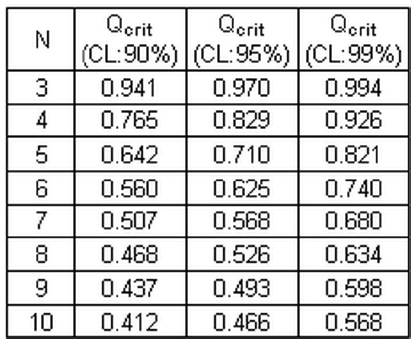
\includegraphics[width=0.5\linewidth]{images/DixonQTestTables}
	\caption{}
	\label{fig:dixonqtesttables}
\end{figure}

\textit{Here: N is the sample size.}
%% - \end{frame}

\begin{itemize}
	\item	With 10 observations and at 90\% confidence, $Q_{Test} = 0.455 > 0.412 =Q_{CV}$ , so we conclude 0.167 is an outlier.
	\item  However, at 95\% confidence, $Q_{Test} = 0.455 < 0.466$ = $Q_{CV}$ 0.167 is not considered an outlier. 
	
	\item This means that for this example we can be 90\% sure that 0.167 is an outlier, but we cannot be 95\% sure.
	\bigskip
	\item (Remark 95\% confidence is equivalent to 5\% signifificance)
\end{itemize}	

\subsection{Testing Outliers with \texttt{R}}
\begin{itemize}
	\item The tests for outliers come in a contributed package called
	“\textbf{outliers}”.
	\item In order to use it one has to download the package to
	the computer. 
	\item It can be done for the command line by using
	\texttt{install.package("outliers")}, otherwise by using a
	convenient interface of the software (Rstudio).
\end{itemize}

%% - \end{frame}
%==================================================================%

Hypothesis for (main variant of) Grubbs' Test and the Dixon Test.

\begin{itemize}
	\item[$H_0$] No Outlier Present in Data
	\item[$H_1$] There is an Outlier Present in Data
\end{itemize}
\bigskip
(\textbf{Important} - Only main variant of Grubbs' Test will be considered when using R )
%% - \end{frame}
%==================================================================%
\subsection{Grubbs Test}
\begin{framed}
	\begin{verbatim}
	x=c(0.403,0.410,0.401,0.380,
	0.400,0.413,0.408)
	grubbs.test(x)
	# Grubbs test for one outlier
	# data: x
	# G = 1.4316, U = 0.0892
	#       p-value = 0.09124
	# alternative hypothesis: 
	lowest value 0.38 is an outlier
	\end{verbatim}
\end{framed}
%% - \end{frame}

%==================================================================%
\subsection{Dixon Test}
\begin{framed}
	\begin{verbatim}
	x=c(0.403,0.410,0.401,0.380,
	0.400,0.413,0.408)
	dixon.test(x)
	
	# Dixon test for outliers
	#data: x
	#Q = 0.7, p-value = 0.1721
	#alternative hypothesis: 
	lowest value 0.38 is an outlier
	\end{verbatim}
\end{framed}
%% - \end{frame}


%=======================================================%


%McBane[1] notes: Dixon provided related tests intended to search for more than one outlier, but they are much less frequently used than the r10 or Q version that is intended to eliminate a single outlier.
%% - http://stats.stackexchange.com/questions/1519/on-univariate-outlier-tests-or-dixon-q-versus-grubbs
%% - http://www.qualitydigest.com/inside/quality-insider-column/problem-outlier-tests.html
%% - http://stats.stackexchange.com/questions/28180/tests-for-univariate-outliers-have-dixons-and-grubbs-methods-been-discredited

%==================================================================%
\subsection{Limitations}
\begin{itemize}
	\item Most of the test in the "outliers" package are designed for small samples. 
	% See also the Rnews article published in May 2006 (vol 6/2) called "processing data for outliers" by Lukasz Komsta (the developer of the package). 
\end{itemize}
%% - \end{frame}
%==================================================================%
\end{document}
